\section{Results and Tests}

Measurements were done for both the polling based system \ref{subsection:polling} and the low energy mode based system \ref{subsection:low-energy}. A repeat pattern of button presses were executed in each mode, and measured.

The sequence is as follows:
\begin{enumerate}
\item
	Press one, two, three and then all buttons simultaneously, and release them one by one.
\item
	Press all buttons at once
\item
	Press one button, and release, twice
\end{enumerate}

\subsection{Polling based system}

As can be seen in the figure \ref{fig:polling-based-system}, the system uses a significant amount of power.
There is a slight spike when buttons are pressed, but the increased amount of power draw is negligible compared to the average draw.

The power usage when the program is running averages about 3.6 $mA$

\begin{figure}[h]
\centering
\includegraphics[width=\textwidth]{figures/polling.pdf}
\caption{Polling based system}
\label{fig:polling-based-system}
\end{figure}

\subsection{Low energy mode based system}
In figure \ref{fig:sleep-based-system}, the difference in power consumption between the times the processor is sleeping, and when buttons are pressed is easily visible.
Some variance in the measurements are visible, these are due to transients as the voltage settles to its new value.

The power usage when the program is sleeping averages about 1.8 ${\mu}A$.

\begin{figure}[h]
\centering
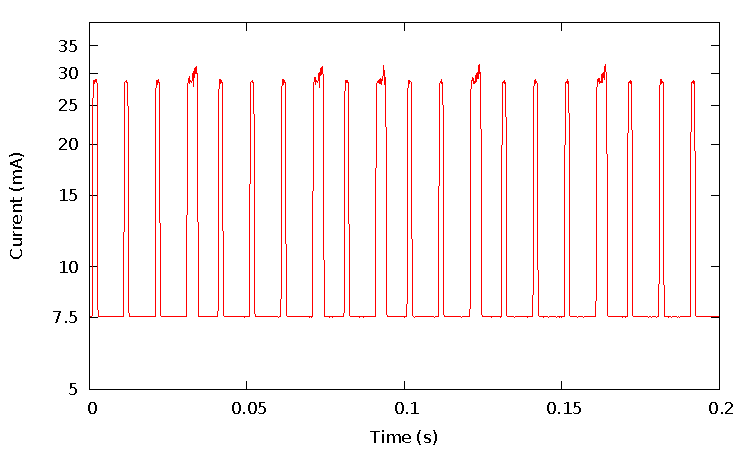
\includegraphics[width=\textwidth]{figures/sleep.pdf}
\caption{Sleep based system}
\label{fig:sleep-based-system}
\end{figure}

\pagebreak

\subsection{System comparison}

The system comparison in figure \ref{fig:system-comparison} easily shows the gains of using a low energy mode when idling. The power draw is different by an order of magnitude. If the systems were to idle, powered only by a 90 $mAh$ coin cell battery, the systems would have a lifetime of fourteen years for the sleeping system, and a single day for the polling one.

The gains of sleeping are considerable.

\begin{figure}[h]
\centering
\includegraphics[width=\textwidth]{figures/all.pdf}
\caption{System comparison}
\label{fig:system-comparison}
\end{figure}

\subsection{Automated testing}

For easier reproducibility, an automatic hardware testing equipment is beneficial. Manual reproduction of testing patterns is prone to error, and large-scale testing is infeasible with manual input.

For those who don't have thousand-dollar equipment at hand, one could attach a micro controller loaded with output sequences to the system, which would then emulate the desired game pad button sequence.